\documentclass[10pt]{beamer}

\usepackage[utf8]{inputenc}
\usepackage[brazil]{babel}
\usepackage{graphicx}		% utilizado para inserir gráfico

% Usado para incluir código
\usepackage{listings}

\usetheme{Copenhagen}
\usecolortheme{lccv}
\setbeamertemplate{background}{
\includegraphics[width=\paperwidth]{./figuras/background_lccv.jpg}}
%\setbeamercovered{transparent}

\title[]{Shell Script Security: Introdução, Conceitos e Técnicas}
\author[]{Baltazar Tavares Vanderlei}
\date{\today}
\institute[2012]{Laboratório de Computação Científica e Visualização - LCCV/UFAL}

\begin{document}

\newcommand{\til}{\~{}}

\frame{\titlepage}
	\begin{frame}[t]
	\frametitle{Sumário}
	\tableofcontents[framebreaks]
	%\tableofcontents[pausesections]
\end{frame}

% Perfumaria sobre o sumário ser mostrado a cada passagem de sessão e sub-sessão.
\AtBeginSection[]{
	\begin{frame}[t]
	\frametitle{Sumário}
	\tableofcontents[currentsection]
	\end{frame}
}

\AtBeginSubsection[]{
	\begin{frame}[t]
	\frametitle{Sumário}
	\tableofcontents[currentsubsection]
	\end{frame}
}

%
% Coisas uteis:
%	* find
%		-> suid
%		-> dev
%		-> time
%		-> delete
%	* tail
%		-> -f
%	* getent
%		-> passwd
%		-> group
%		-> 3 field(retorno de erro)
%	* IFS
%		-> exemplo com IP
%		-> usando como cut
%		-> em while
%
% Seguranca em ling. bash:
%	* eval is the root of all evil
%	* sempre use '"'
%		-> exemplo, com eval(?)
%


\section{Tornando a vida mais facil e segura}
	\subsection{Usando o find}
		\begin{frame}%[t]
		\frametitle{O que podemos fazer com o find?}
			\begin{itemize}[<+->]
				\item Basicamente podemos pesquisar
				\item Todo o tipo de pesquisa pode ser feito no find
				\item Por tipos, tamanho e outras caratecteristicas
			\end{itemize}
		\end{frame}

		\begin{frame}%[t]
		\frametitle{Vamos aumentar um pouco nossa seguranca, eliminando suid}
			\lstinputlisting[language=bash]{./codigo/find_suid.sh}
		\end{frame}

		\begin{frame}%[t]
		\frametitle{Procurando por tamanho:}
			\lstinputlisting[language=bash]{./codigo/find_size.sh}
		\end{frame}

		\begin{frame}%[t]
		\frametitle{Procurando por tempo:}
			\lstinputlisting[language=bash]{./codigo/find_ctime.sh}
		\end{frame}

		\begin{frame}%[t]
		\frametitle{Deletando: pondo em pratica}
			\lstinputlisting[language=bash]{./codigo/find_delete.sh}
		\end{frame}

%	* tail
%		-> -f

%	\subsection{Desafios}
		\begin{frame}%[t]
		\frametitle{Desafios como membro da GradeBR}
			\begin{block}{Desafio}
				Usar tecnologia de ponta para planejar e implementar um grid de processamento de alto desempenho, que pudesse processar problemas de escala peta(da escala de $10^{15}$) de forma cooperativa entre os vários nós.
			\end{block}
		\end{frame}

\section{O que um nó da GradeBR precisa?}
		\begin{frame}%[t]
		\frametitle{Necessario:}
			\begin{itemize}%[<+->]
				% pergunta
				\item Grande poder de processamento e memória
				\item Grande espaço e velocidade de armazenamento
				\item Uma rede de interconexão extremamente mais rápida que a convencional
				\item Um sistema tolerante a falhas, robusto e funcional(tanto em hardware como em software)
			\end{itemize}
		\end{frame}

\section{Poder de processamento e memória}
		\begin{frame}%[t]
		\frametitle{O cluster do LCCV possui:}
			\begin{itemize}%[<+->]
				\item \textbf{8} placas de vídeo totalizando \textbf{30}Tflops
				\item \textbf{218} nós de processamento, com processadores \textbf{i7}
				\item Cada maquina com \textbf{2} processadores, cada processador \textbf{4} núcleos
				\item Cada maquina com \textbf{24}GB de memória NUMA
				\item Totalizando mais de \textbf{5}TB de memória NUMA e \textbf{1744} núcleos
				\item Só de nós de processamento, temos \textbf{20 Tflops}
			\end{itemize}
		\end{frame}

		\begin{frame}%[t]
		\frametitle{Blades:}
			\begin{figure}
			\centering
				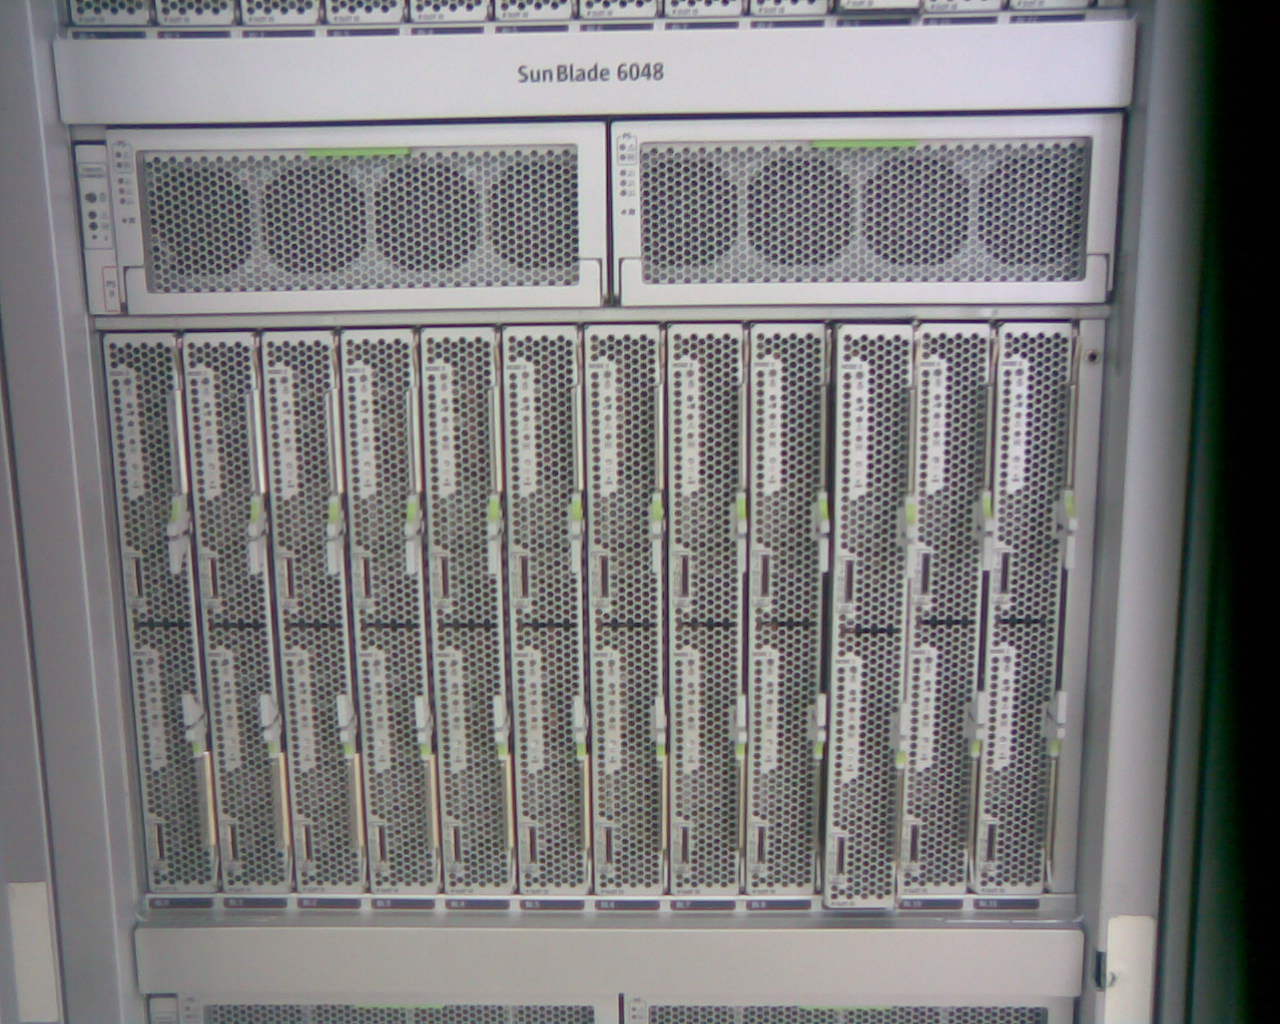
\includegraphics[scale=0.15]{./figuras/gaveta_blades.jpg}
			\end{figure}
		\end{frame}

		\begin{frame}%[t]
		\frametitle{Blades:}
			\begin{figure}
			\centering
				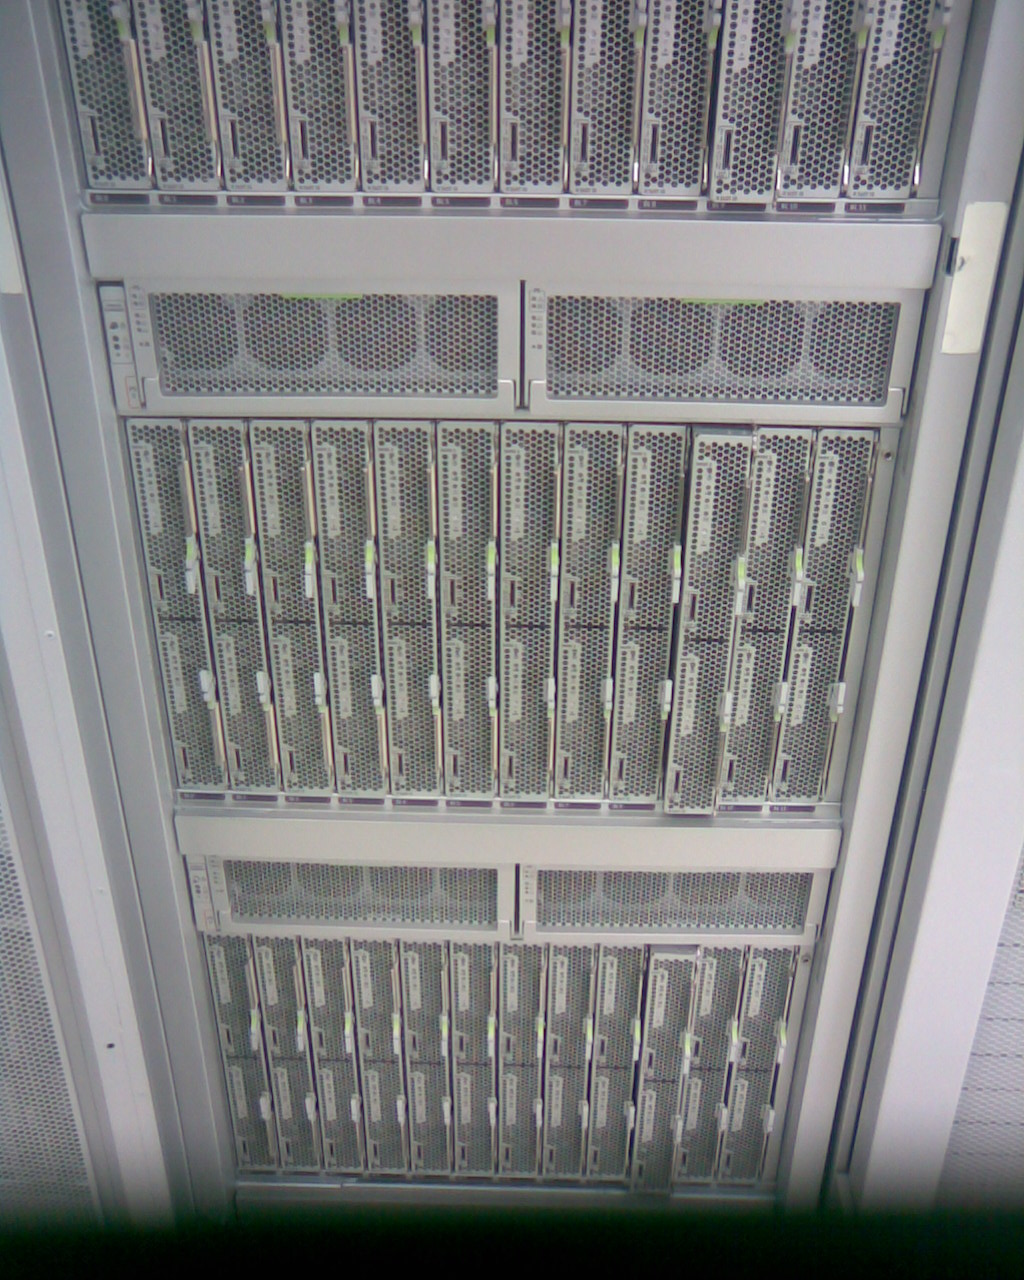
\includegraphics[scale=0.15]{./figuras/rack.jpg}
			\end{figure}
		\end{frame}

		\begin{frame}%[t]
		\frametitle{Blades:}
			\begin{figure}
			\centering
				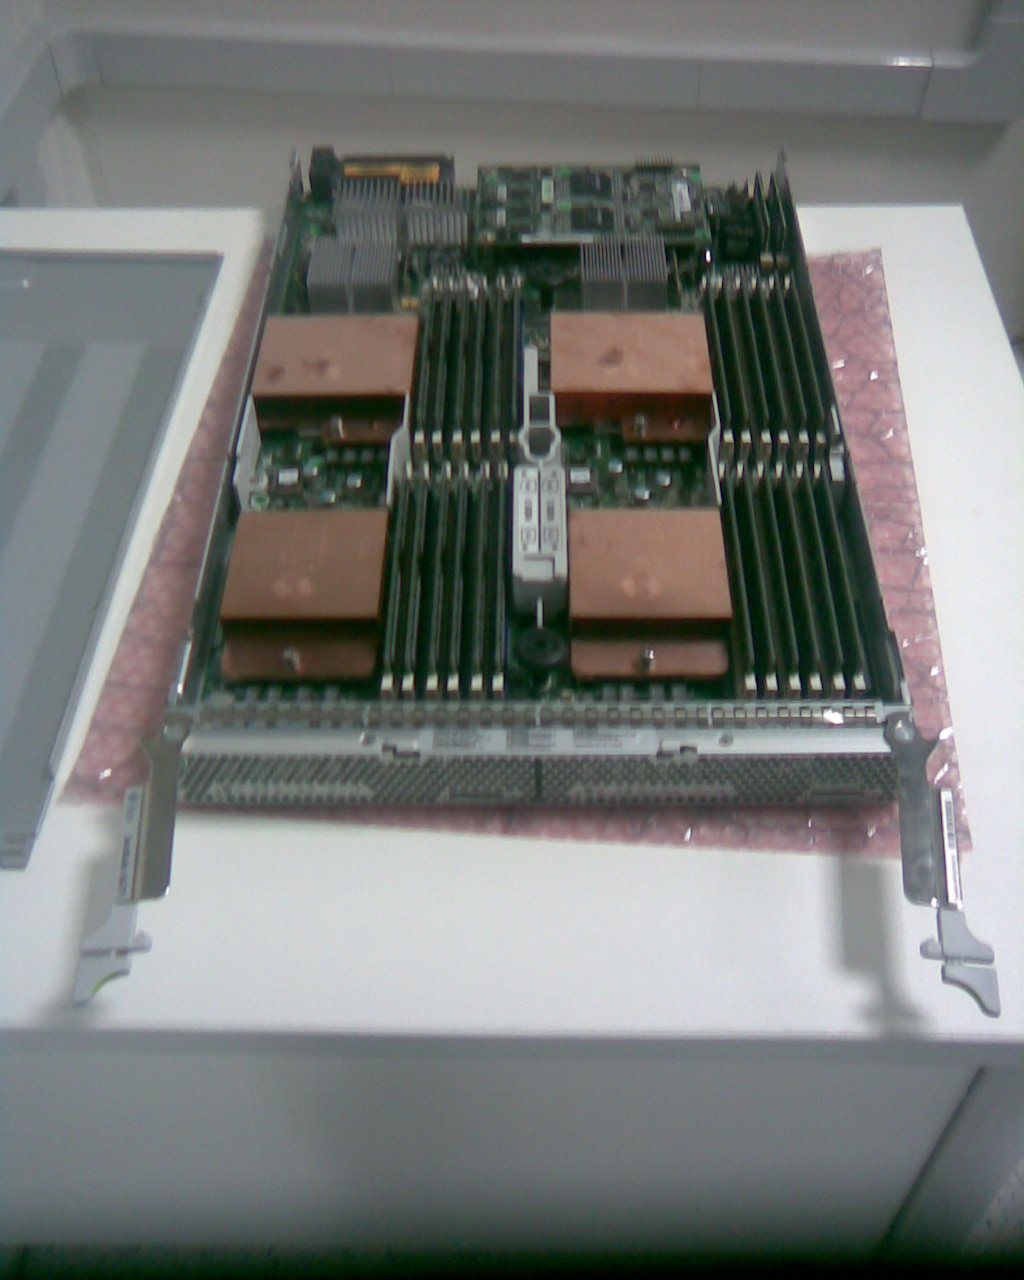
\includegraphics[scale=0.15]{./figuras/img_blade.jpg}
			\end{figure}
		\end{frame}

		\begin{frame}%[t]
		\frametitle{Blades:}
			\begin{figure}
			\centering
				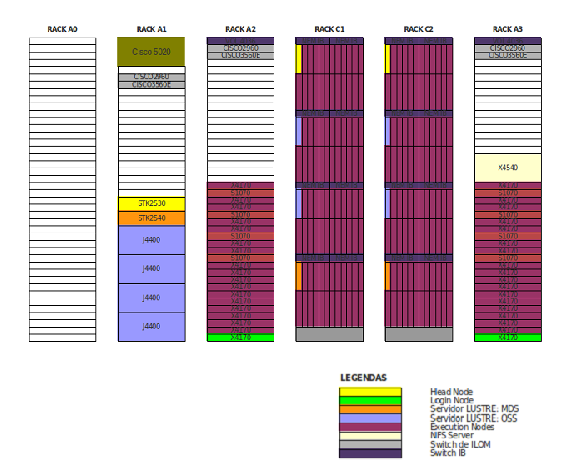
\includegraphics[width=0.9\textwidth]{./figuras/mapa_racks.png}
			\end{figure}
		\end{frame}

\section{Rede de interconexão de alto desempenho}
%	\subsection{InfiniBand}
	\begin{frame} %[t]
	\frametitle{Porque foi escolhida essa topologia e interconexão}
		\begin{itemize}[<+->]
			\item Para a rede de alto desempenho, foi escolhido o InfiniBand(IB)
			\item O IB é um meio com baixa latência
			\item Tem uma alta taxa de transferência
			\item É usado para conexão entre maquinas(compatível com MPI)
			\item É usado por dispositivos de armazenamento(compatível com o lustre)
			\item Pode ser usada uma camada de compatibilidade com o IP(chamada de ``IPoIB")
			\item Com IB, foi conseguido uma taxa de transferência máxima de 40Gbit/s
		\end{itemize}
	\end{frame}

	\begin{frame}%[t]
	\frametitle{Topologia adotada:}
		\begin{figure}
		\centering
			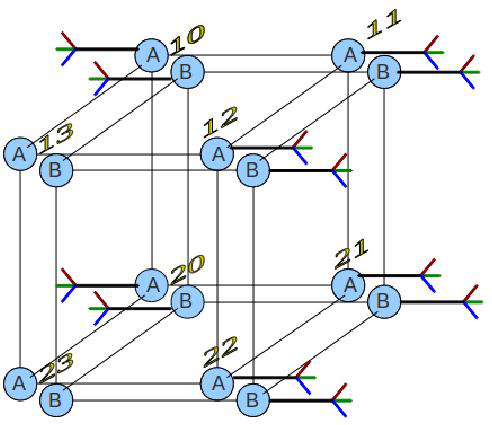
\includegraphics[scale=0.5]{./figuras/hipercubo.png}
			\caption{hipercubo 4D}
		\end{figure}
	\end{frame}


\section{Armazenamento de alto desempenho}
	\begin{frame} %[t]
	\frametitle{Para armazenamento de alto desempenho, era nescessário:}
		\begin{itemize}[<+->]
			\item Um sistema de arquivo que funcionasse via rede
			\item Um sistema de arquivo paralelo
			\item Escalável para um grande numero de clientes
			\item Compatível com o hardware usado
		\end{itemize}
	\end{frame}

	\begin{frame}
	\frametitle{Porque foi escolhido o lustrefs:}
		\begin{itemize}[<+->]
			\item Sistema de arquivos via rede e paralelo
			\item Possível usar raid e garantir segurança e acesso rápido a dados
			\item Escalável ate dezenas de milhares de clientes
			\item Suporte a IB, usando rdma para se comunicar diretamente
			\item Tolerância a falhas e Alta disponibilidade(sem balanço de carga)
		\end{itemize}
	\end{frame}

\section{Características do Sistema}
	\begin{frame}
	\frametitle{O que aumenta a dificuldade com o sistema:}
		\begin{itemize}[<+->]
			\item Um sistema com muitos clientes
			\item Alta disponibilidade e balanço de carga em serviços
			\item Lidar com o sistema de varias maquinas ao mesmo tempo
			\item Lidar com programas escalonadores
			\item Vários problemas por lidar com tecnologia de ponta
			\item Sistema muito grande e complexo
		\end{itemize}
	\end{frame}

\section{Conclusão}
	\subsection{Benchmarks}
%	\subsection{HPL}
		\begin{frame}
		\frametitle{HPL:}
			\begin{block}{O que é o HPL?}
				HPL é um teste amplamente usado que mede a eficiência de um cluster em flops.
			\end{block}
			\begin{itemize}%[<+->]
				\item O Cluster teve um resultado de 17TFlops.
				\item Resultados parciais com eficiência superior a 85\%($R_{max}/R_{peak}$).
			\end{itemize}
		\end{frame}

%	\subsection{IOR}
		\begin{frame}
		\frametitle{IOR:}
			\begin{block}{O que é o IOR?}
				IOR é um teste usado que mede a escrita e leitura de um cluster em um sistema de arquivos usando posix e mpi-io.
			\end{block}
			\begin{table}[htb] % [htb]-> here, top, bottom
				\centering   % tabela centralizada
				\large       % tamanho da fonte 
				\setlength{\arrayrulewidth}{2\arrayrulewidth}  % espessura da  linha
				\setlength{\belowcaptionskip}{10pt}  % espaço entre caption e tabela
				\caption{\it Resultados do IOR}
				\begin{tabular}{|c|c|c|c|} % c=center, l=left, r=right 
					\hline
					POSIX [GB/s] & MPI-IO [GB/s] \\
					\hline \hline
					Leitura | Escrita  & Leitura \\
					\hline \hline
					6,8 | 2,7 & 6 \\
					\hline
				\end{tabular}
				\label{tab:res_ior}
			\end{table}
		\end{frame}

	\subsection{Estado atual}
	\begin{frame}
	\frametitle{Estado atual}
		\begin{itemize}[<+->]
			\item Um dos maiores supercomputadores em atividade na América Latina
			\item Foram executadas mais de 500 mil horas de processamento em projetos do LCCV/Petrobras
			\item Implementamos com sucesso um cluster de alto desempenho
			\item Preparando a infraestrutura para o grid continental de alto desempenho GradeBR
		\end{itemize}
	\end{frame}

	\begin{frame}
	\frametitle{Agradecimentos}
		\begin{block}{}%{Agradecimento}
			Agradecemos a ANP, a Petrobras e ao Laboratório de Computação Científica e Visualização da Universidade Federal de Alagoas por garantir acesso aos recursos computacionais do cluster GradeBR/UFAL da Rede Galileu.
		\end{block}
	\end{frame}
\end{document}

